% !TEX root =  GroupDet.tex

\section{Descriptor Metric Learning}
\label{MetLearn}

As mentioned in Section \ref{agg}, we learn matrices $\Sigma_{I}$, $\Sigma_{P}$ for the Mahalanobis distances $d_I(\mathbf{f},\mathbf{f}')$ and $d_P(\mathbf{g},\mathbf{g}')$, so that the learned metrics can 1) enhance discrimination between exemplar categories by ensuring that distances are smaller when descriptors are drawn from roughly the same temporal location within a labeled exemplar of the same category, and larger otherwise; and 2) enhance the accuracy of temporal localization by ensuring that distances between labeled ensembles and unlabeled ``background'' ensembles are large. Such metrics not only help the participants represented by the optimal matching matrix $W^{*}$ to emerge, as discussed in \ref{vote}, but also enable efficient temporal localization by branch-and-bound, as required in \ref{BB}. We achieve these objectives simultaneously using an adaptation of the Large Margin Nearest Neighbor (LMNN) framework~\cite{Weinberger:ML}. 

For each application, we use as training set the exemplar videos, possibly with different numbers of agents $N$, with each exemplar annotated with start/end times. ``ground-truth"matching, and a category label. We use unlabeled time units in the videos as ``background'' samples. Intuitively, the learned metrics should satisfy the six types of constraints shown in Fig.~\ref{ML_illustration}. This figure depicts three different exemplar videos in which a subset of time units have been labeled as being distinctive interactions of two different classes. In this example, each labeled exemplar is shown as being divided into two cells; these correspond to the lowest level of the temporal pyramid described in Section~\ref{BB}. The first three constraints in the list enhance discrimination between categories, while the last three enhance the accuracy of temporal localization. Offsetting all of the distances by $-1$ ensures that the function $q(t)$ in (\ref{qfunction}) assumes a negative value as required for branch-and-bound search. 

\begin{figure}[t]
\begin{centering}
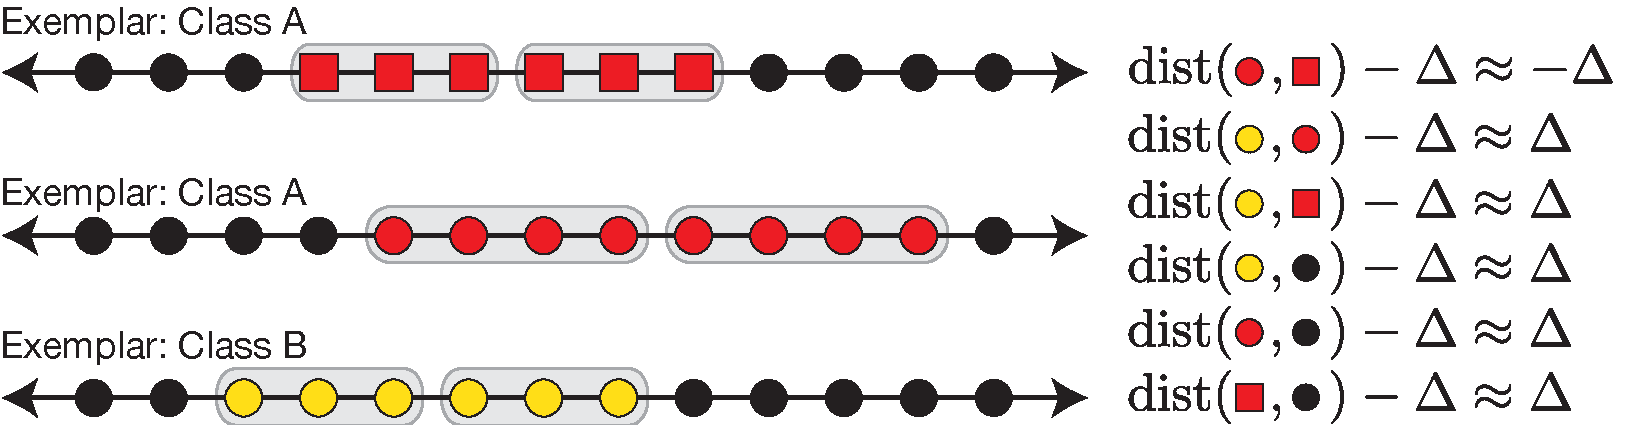
\includegraphics[width=\columnwidth]{metriclearning}
\end{centering}
\caption{Constraints used in discriminative metric learning. Each row is a labeled two-cell exemplar with markers representing instantaneous descriptor-ensembles at each time unit. For discrimination between interaction categories, distances between ensembles of the same class (red circles and red squares) should be small whenever they occur in the same cell number; and distances for different classes (red vs. yellow) should be large. For efficient temporal localization, distances between ensembles at labeled times and unlabeled ``background'' times (black circles) should also be large.\ruonan{The $d$'s have to be changed into $D$'s or $\hat{D}$'s, neither of which is perfect. It is because the annotation also include the ground-truth matching/correspondence between agents from two training exemplars, and metric learning must use this ground-truth matching as well (please see Eq. (\ref{classify})). The ground-truth matching however has not been visualized and might be cumbersome to visualize... }}
\label{ML_illustration}
\end{figure}

We enforce these constraints through an LMNN framework by construct two different types of collections from our database exemplars. The first collection $\mathcal{P}$ contains all pairs of instantaneous interaction ensembles that are of the same category (red circles and red squares in Fig.~\ref{ML_illustration}) and occur roughly in the same temporal location within the interaction instances (\ie, in the same cell of the lowest level of the temporal pyramids). The second collection $\mathcal{M}$ is comprised of ordered triples $(h,k,l)$ in which ensemble $h$ is the same category as ensemble $k$ and ensemble $l$ is either of a different category or background. It is also useful to add to collection $\mathcal{M}$ additional triples in which $l$ is derived from same-category same-cell pairs but with permuted incorrect matching matrices. Having defined these two collections, each Mahalanobis metric is found by solving
\begin{equation}
\label{classify}
\begin{split}
&\min_{\Sigma_{I}, \Sigma_{P}} \sum_{(u,v)\in\mathcal{P}}\hat{D}(\mathcal{D}_{u}, \mathcal{D}_{v}, W_{u,v})+\gamma\sum_{(h,k,l)\in\mathcal{M}}\xi_{h,k,l}\\
&\textup{s.t.}  \hat{D}(\mathcal{D}_{h}, \mathcal{D}_{l}, W_{h,l})-\hat{D}(\mathcal{D}_{h}, \mathcal{D}_{k}, W_{h,k})\ge 2-\xi_{h,k,l}'\\
&\xi_{h,k,l}\ge0, \Sigma_{I}\succeq 0, \Sigma_{P}\succeq 0,
\end{split}
\end{equation}
where the minimization over either $\Sigma_{I}$ or $\Sigma_{P}$ exactly falls into the framework of LMNN \cite{Weinberger:ML}. Therefore, We apply LMNN multiple times to separately learn one distinct pair of ($\Sigma_{I}, \Sigma_{P}$) for each value of $N$ that exists in the training set. 


%Recall that 1) in Section \ref{vote} we expect the score $D$ to be small when a temporal unit in the input is best aligned to a temporal unit in the exemplar by the `correct' matching matrix; and 2) in Section \ref{BB} we expect the dissimilarity $D^{*}(t)$ are driven toward zero in the `ground-truth' interval $[t_{s}, t_{e}]$ , and toward a large positive number $2\Delta$ otherwise. For both purposes, we learn an effective ensemble dissimilarity measure. Recall that the ensemble dissimilarity $D$ or $\hat{D}$ is aggregated from `atomic' descriptor distances $\{ d_{I}(\mathbf{f}_{m,t}, \mathbf{f}^{D}_{n,s}), d_{P}(\mathbf{g}_{m,m',t}, \mathbf{g}^{D}_{n,n',s})\}$, and the ensemble dissimilarity learning therefore narrows down to learning effective `atomic'  distances.  We parameterize an atomic distance by a Mahalanobis metric, \textit{i.e.}, let $d_{I}(\mathbf{f}, \mathbf{f}')=(\mathbf{f}-\mathbf{f}')^{T}\Sigma_{I}(\mathbf{f}-\mathbf{f}')$ and $d_{P}(\mathbf{g}, \mathbf{g}')=(\mathbf{g}-\mathbf{g}')^{T}\Sigma_{P}(\mathbf{g}-\mathbf{g}')$, where $\Sigma_{I}\succeq 0$ and $\Sigma_{P}\succeq 0$ are positive semi-definite matrices.  
%
%We learn each pair of Mahalanobis metrics $(\Sigma_{I}, \Sigma_{P})$ for each number of participants separately. To do so, we construct two different types of collections from our database exemplars. The first collection, $\mathcal{P}$, contains all pairs of instantaneous interaction ensembles that are similar to each other. The second collection, $\mathcal{M}$, is comprised of all ordered triples $(h,k,l)$ in which ensemble $h$ is similar to ensemble $k$ but they two  are dissimilar to ensemble $l$. In the present case, we build the collection $\mathcal{P}$ and the ($(h,k)$-indexed) similar pairs in collection $\mathcal{M}$ using all instantaneous ensemble pairs with their ground-truth matching matrices from the same category extracted from the same cell at the lowest level of the pyramid. Similarly, we include in the ($(h,l)$-indexed and $(k,l)$-indexed) dissimilar pairs of collection $\mathcal{M}$ the ensembles extracted from: 1) different-category exemplars; 2) same-category same-cell ensembles with simulated wrong matching matrices; and 3) ensembles within interaction intervals against ensembles from `background' non-interaction intervals. Eventually, we find the Mahalanobis metrics by solving
%\begin{equation}
%\label{classify}
%\begin{split}
%&\min_{\xi_{h,k,l}\ge0, \Sigma_{I}\succeq 0, \Sigma_{P}\succeq 0} \sum_{(u,v)\in\mathcal{P}}\hat{D}(\mathcal{D}_{u}, \mathcal{D}_{v}, W_{u,v})+\gamma\sum_{(h,k,l)\in\mathcal{M}}\xi_{h,k,l}\\
%&\textup{s.t.}  \hat{D}(\mathcal{D}_{h}, \mathcal{D}_{l}, W_{h,l})-\hat{D}(\mathcal{D}_{h}, \mathcal{D}_{k}, W_{h,k})\ge 2\Delta-\xi_{h,k,l}.
%\end{split}
%\end{equation}
%Note that $\Delta$ is the large positive number as used in (\ref{quality}), and (\ref{classify}) will encourage a similar pair to contribute a negative summand around $-\Delta$ to (\ref{quality}), and encourage a dissimilar pair to contribute approximately $+\Delta$ summand,  thus enabling the branch-and-bound search as introduced in Section \ref{BB}.  The minimization over either $\Sigma_{I}$ or $\Sigma_{P}$ falls into the framework of large margin nearest neighbor (LMNN) formulation \cite{Weinberger:ML}, and we simply decompose (\ref{classify}) into independent LMNN tasks and employ \cite{Weinberger:ML}.
